\documentclass[]{article}
\usepackage{lmodern}
\usepackage{amssymb,amsmath}
\usepackage{ifxetex,ifluatex}
\usepackage{fixltx2e} % provides \textsubscript
\ifnum 0\ifxetex 1\fi\ifluatex 1\fi=0 % if pdftex
  \usepackage[T1]{fontenc}
  \usepackage[utf8]{inputenc}
\else % if luatex or xelatex
  \ifxetex
    \usepackage{mathspec}
  \else
    \usepackage{fontspec}
  \fi
  \defaultfontfeatures{Ligatures=TeX,Scale=MatchLowercase}
\fi
% use upquote if available, for straight quotes in verbatim environments
\IfFileExists{upquote.sty}{\usepackage{upquote}}{}
% use microtype if available
\IfFileExists{microtype.sty}{%
\usepackage{microtype}
\UseMicrotypeSet[protrusion]{basicmath} % disable protrusion for tt fonts
}{}
\usepackage[margin=1in]{geometry}
\usepackage{hyperref}
\hypersetup{unicode=true,
            pdftitle={Random effect multinomial model},
            pdfauthor={A. J. Rominger},
            pdfborder={0 0 0},
            breaklinks=true}
\urlstyle{same}  % don't use monospace font for urls
\usepackage{color}
\usepackage{fancyvrb}
\newcommand{\VerbBar}{|}
\newcommand{\VERB}{\Verb[commandchars=\\\{\}]}
\DefineVerbatimEnvironment{Highlighting}{Verbatim}{commandchars=\\\{\}}
% Add ',fontsize=\small' for more characters per line
\usepackage{framed}
\definecolor{shadecolor}{RGB}{248,248,248}
\newenvironment{Shaded}{\begin{snugshade}}{\end{snugshade}}
\newcommand{\KeywordTok}[1]{\textcolor[rgb]{0.13,0.29,0.53}{\textbf{{#1}}}}
\newcommand{\DataTypeTok}[1]{\textcolor[rgb]{0.13,0.29,0.53}{{#1}}}
\newcommand{\DecValTok}[1]{\textcolor[rgb]{0.00,0.00,0.81}{{#1}}}
\newcommand{\BaseNTok}[1]{\textcolor[rgb]{0.00,0.00,0.81}{{#1}}}
\newcommand{\FloatTok}[1]{\textcolor[rgb]{0.00,0.00,0.81}{{#1}}}
\newcommand{\ConstantTok}[1]{\textcolor[rgb]{0.00,0.00,0.00}{{#1}}}
\newcommand{\CharTok}[1]{\textcolor[rgb]{0.31,0.60,0.02}{{#1}}}
\newcommand{\SpecialCharTok}[1]{\textcolor[rgb]{0.00,0.00,0.00}{{#1}}}
\newcommand{\StringTok}[1]{\textcolor[rgb]{0.31,0.60,0.02}{{#1}}}
\newcommand{\VerbatimStringTok}[1]{\textcolor[rgb]{0.31,0.60,0.02}{{#1}}}
\newcommand{\SpecialStringTok}[1]{\textcolor[rgb]{0.31,0.60,0.02}{{#1}}}
\newcommand{\ImportTok}[1]{{#1}}
\newcommand{\CommentTok}[1]{\textcolor[rgb]{0.56,0.35,0.01}{\textit{{#1}}}}
\newcommand{\DocumentationTok}[1]{\textcolor[rgb]{0.56,0.35,0.01}{\textbf{\textit{{#1}}}}}
\newcommand{\AnnotationTok}[1]{\textcolor[rgb]{0.56,0.35,0.01}{\textbf{\textit{{#1}}}}}
\newcommand{\CommentVarTok}[1]{\textcolor[rgb]{0.56,0.35,0.01}{\textbf{\textit{{#1}}}}}
\newcommand{\OtherTok}[1]{\textcolor[rgb]{0.56,0.35,0.01}{{#1}}}
\newcommand{\FunctionTok}[1]{\textcolor[rgb]{0.00,0.00,0.00}{{#1}}}
\newcommand{\VariableTok}[1]{\textcolor[rgb]{0.00,0.00,0.00}{{#1}}}
\newcommand{\ControlFlowTok}[1]{\textcolor[rgb]{0.13,0.29,0.53}{\textbf{{#1}}}}
\newcommand{\OperatorTok}[1]{\textcolor[rgb]{0.81,0.36,0.00}{\textbf{{#1}}}}
\newcommand{\BuiltInTok}[1]{{#1}}
\newcommand{\ExtensionTok}[1]{{#1}}
\newcommand{\PreprocessorTok}[1]{\textcolor[rgb]{0.56,0.35,0.01}{\textit{{#1}}}}
\newcommand{\AttributeTok}[1]{\textcolor[rgb]{0.77,0.63,0.00}{{#1}}}
\newcommand{\RegionMarkerTok}[1]{{#1}}
\newcommand{\InformationTok}[1]{\textcolor[rgb]{0.56,0.35,0.01}{\textbf{\textit{{#1}}}}}
\newcommand{\WarningTok}[1]{\textcolor[rgb]{0.56,0.35,0.01}{\textbf{\textit{{#1}}}}}
\newcommand{\AlertTok}[1]{\textcolor[rgb]{0.94,0.16,0.16}{{#1}}}
\newcommand{\ErrorTok}[1]{\textcolor[rgb]{0.64,0.00,0.00}{\textbf{{#1}}}}
\newcommand{\NormalTok}[1]{{#1}}
\usepackage{graphicx,grffile}
\makeatletter
\def\maxwidth{\ifdim\Gin@nat@width>\linewidth\linewidth\else\Gin@nat@width\fi}
\def\maxheight{\ifdim\Gin@nat@height>\textheight\textheight\else\Gin@nat@height\fi}
\makeatother
% Scale images if necessary, so that they will not overflow the page
% margins by default, and it is still possible to overwrite the defaults
% using explicit options in \includegraphics[width, height, ...]{}
\setkeys{Gin}{width=\maxwidth,height=\maxheight,keepaspectratio}
\IfFileExists{parskip.sty}{%
\usepackage{parskip}
}{% else
\setlength{\parindent}{0pt}
\setlength{\parskip}{6pt plus 2pt minus 1pt}
}
\setlength{\emergencystretch}{3em}  % prevent overfull lines
\providecommand{\tightlist}{%
  \setlength{\itemsep}{0pt}\setlength{\parskip}{0pt}}
\setcounter{secnumdepth}{0}
% Redefines (sub)paragraphs to behave more like sections
\ifx\paragraph\undefined\else
\let\oldparagraph\paragraph
\renewcommand{\paragraph}[1]{\oldparagraph{#1}\mbox{}}
\fi
\ifx\subparagraph\undefined\else
\let\oldsubparagraph\subparagraph
\renewcommand{\subparagraph}[1]{\oldsubparagraph{#1}\mbox{}}
\fi

%%% Use protect on footnotes to avoid problems with footnotes in titles
\let\rmarkdownfootnote\footnote%
\def\footnote{\protect\rmarkdownfootnote}

%%% Change title format to be more compact
\usepackage{titling}

% Create subtitle command for use in maketitle
\newcommand{\subtitle}[1]{
  \posttitle{
    \begin{center}\large#1\end{center}
    }
}

\setlength{\droptitle}{-2em}
  \title{Random effect multinomial model}
  \pretitle{\vspace{\droptitle}\centering\huge}
  \posttitle{\par}
  \author{A. J. Rominger}
  \preauthor{\centering\large\emph}
  \postauthor{\par}
  \predate{\centering\large\emph}
  \postdate{\par}
  \date{12 May 2017}


\begin{document}
\maketitle

\section{The model}\label{the-model}

Given the number of sequencing reads assigned to each of \(S\) species,
we want to estimate the number of individuals for each species that went
into the sequencing run, call that vector \(x\). We know the total
number of reads \(N_{reads}\), the number of species \(S\), the total
number of individuals \(N\) that were sequenced, and the vector of
number of reads per species \(x_{read}\). We assume that stochastic
evolutionary processes have led to some species having a greater
propensity to be sequenced. These stochastic processes we summarize in a
random effect \(nu\). We further assume that within orders these random
effects are constant, thus each species within the same order gets the
same random effect.

Thus our model for the number of reads is: \[
x_{reads} \sim \text{multinom}\left(N_{reads}, \frac{x\nu}{\sum_i x_i \nu_i}\right)
\]

Thus the vector of probabilities for the multinomial distribution is
proportional to the unknown abundance times the unknown random effect
\(\nu\).

We could choose to put a multinomial prior on \(x\) because
\(N = \sum x\) is fixed, or could approximate \(x_i\) with a continuous
prior and assume \(N\) is large enough such that
\(Cov(x_i, x_j) \approx 0\). Allowing \(x_i\) to be iid and continuous
allows us to better estimate the relative contribution of \(x\) and
\(\nu\) in determining \(x_{reads}\), so we opt for the prior: \[
\text{log}(x_i) \sim norm\left(\frac{N}{S}, \sigma^2_x\right)
\]

Given that \(\nu\) is constant within orders, varies across orders, and
must be positive, we model it as \[
\text{log}(\nu_{order=j}) \sim \text{norm}(0, \sigma^2_{\nu})
\] That is, for order \(j\) the log of the random effect is distributed
normally with mean 0 and variance \(\sigma^2_{\nu}\).

\section{Running the model in JAGS}\label{running-the-model-in-jags}

First we set up the simulation

\begin{Shaded}
\begin{Highlighting}[]
\CommentTok{# number of orders}
\NormalTok{nOrd <-}\StringTok{ }\DecValTok{8}

\CommentTok{# number of species}
\NormalTok{nspp <-}\StringTok{ }\NormalTok{nOrd *}\StringTok{ }\DecValTok{10}

\CommentTok{# vector identifying which species are in which orders}
\NormalTok{ordID <-}\StringTok{ }\KeywordTok{rep}\NormalTok{(}\DecValTok{1}\NormalTok{:nOrd, }\DataTypeTok{each =} \NormalTok{nspp/nOrd)}

\CommentTok{# simulate random effect}
\NormalTok{ordSD <-}\StringTok{ }\FloatTok{0.25}
\KeywordTok{set.seed}\NormalTok{(}\DecValTok{1}\NormalTok{)}
\NormalTok{ordEffect <-}\StringTok{ }\KeywordTok{exp}\NormalTok{(}\KeywordTok{rnorm}\NormalTok{(nOrd, }\DataTypeTok{mean =} \DecValTok{0}\NormalTok{, }\DataTypeTok{sd =} \NormalTok{ordSD))}

\CommentTok{# generate true abundances for each species}
\KeywordTok{set.seed}\NormalTok{(}\DecValTok{1}\NormalTok{)}
\NormalTok{x <-}\StringTok{ }\KeywordTok{sample}\NormalTok{(}\KeywordTok{seq}\NormalTok{(}\DecValTok{1}\NormalTok{, }\DecValTok{80}\NormalTok{, }\DataTypeTok{length.out =} \NormalTok{nspp))}

\CommentTok{# simulate number of reads for each species}
\NormalTok{totReads <-}\StringTok{ }\DecValTok{10}\NormalTok{^}\DecValTok{6}
\KeywordTok{set.seed}\NormalTok{(}\DecValTok{1}\NormalTok{)}
\NormalTok{xreads <-}\StringTok{ }\KeywordTok{rmultinom}\NormalTok{(}\DecValTok{1}\NormalTok{, totReads, x*ordEffect[ordID])[, }\DecValTok{1}\NormalTok{]}
\end{Highlighting}
\end{Shaded}

A quick plot of what those simulated data look like (colors correspond
to order identity)

\begin{Shaded}
\begin{Highlighting}[]
\KeywordTok{palette}\NormalTok{(}\KeywordTok{hsv}\NormalTok{(}\DataTypeTok{h =} \KeywordTok{seq}\NormalTok{(}\DecValTok{0}\NormalTok{, }\FloatTok{0.8}\NormalTok{, }\DataTypeTok{length.out =} \KeywordTok{max}\NormalTok{(ordID)), }
            \DataTypeTok{s =} \DecValTok{1}\FloatTok{-0.3}\NormalTok{*}\KeywordTok{seq}\NormalTok{(-}\DecValTok{1}\NormalTok{, }\DecValTok{1}\NormalTok{, }\DataTypeTok{length.out =} \KeywordTok{max}\NormalTok{(ordID))^}\DecValTok{2}\NormalTok{, }
            \DataTypeTok{v =} \FloatTok{0.7} \NormalTok{+}\StringTok{ }\FloatTok{0.3}\NormalTok{*}\KeywordTok{seq}\NormalTok{(-}\DecValTok{1}\NormalTok{, }\DecValTok{1}\NormalTok{, }\DataTypeTok{length.out =} \KeywordTok{max}\NormalTok{(ordID))^}\DecValTok{2}\NormalTok{, }
            \DataTypeTok{alpha =} \FloatTok{0.7}\NormalTok{))}

\KeywordTok{par}\NormalTok{(}\DataTypeTok{mar =} \KeywordTok{c}\NormalTok{(}\DecValTok{3}\NormalTok{, }\DecValTok{3}\NormalTok{, }\DecValTok{0}\NormalTok{, }\DecValTok{0}\NormalTok{) +}\StringTok{ }\FloatTok{0.5}\NormalTok{, }\DataTypeTok{mgp =} \KeywordTok{c}\NormalTok{(}\DecValTok{2}\NormalTok{, }\FloatTok{0.75}\NormalTok{, }\DecValTok{0}\NormalTok{))}
\KeywordTok{plot}\NormalTok{(x, xreads, }\DataTypeTok{bg =} \NormalTok{ordID, }\DataTypeTok{pch =} \DecValTok{21}\NormalTok{, }
     \DataTypeTok{xlab =} \StringTok{'Abundance'}\NormalTok{, }\DataTypeTok{ylab =} \StringTok{'Number of reads'}\NormalTok{)}
\end{Highlighting}
\end{Shaded}

\begin{center}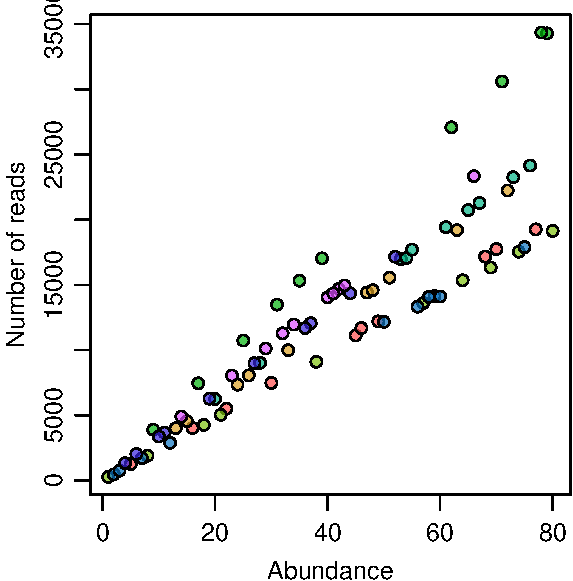
\includegraphics{modelDerivation_normPrior_files/figure-latex/fig_simAbund-1} \end{center}

Define the model in JAGS using \texttt{rjags}

\begin{Shaded}
\begin{Highlighting}[]
\KeywordTok{library}\NormalTok{(rjags)}
\end{Highlighting}
\end{Shaded}

\begin{verbatim}
## Loading required package: coda
\end{verbatim}

\begin{verbatim}
## Linked to JAGS 4.2.0
\end{verbatim}

\begin{verbatim}
## Loaded modules: basemod,bugs
\end{verbatim}

\begin{Shaded}
\begin{Highlighting}[]
\CommentTok{# write the model out}
\KeywordTok{cat}\NormalTok{(}\StringTok{'model\{}
\StringTok{        # reads model}
\StringTok{        xreads[1:S] ~ dmulti(alpha[1:S], totReads)}
\StringTok{    }
\StringTok{        # priors}
\StringTok{        sigX ~ dunif(0, 100)}
\StringTok{        tauX <- 1/(sigX^2)}
\StringTok{        sigCopy ~ dunif(0, 100)}
\StringTok{        tauCopy <- 1/(sigCopy^2)}
\StringTok{    }
\StringTok{        # species-level effect}
\StringTok{        for(i in 1:S) \{}
\StringTok{            logX[i] ~ dnorm(N/S, tauX)}
\StringTok{            x[i] <- exp(logX[i])}
\StringTok{        \}}

\StringTok{        # order-level random effect}
\StringTok{        for(j in 1:nOrd) \{}
\StringTok{            logNu[j] ~ dnorm(0, tauCopy)}
\StringTok{            nu[j] <- exp(logNu[j])}
\StringTok{        \}}
\StringTok{    }
\StringTok{        # define multinom param}
\StringTok{        for(i in 1:S) \{}
\StringTok{            alpha[i] <- x[i] * nu[ordID[i]]}
\StringTok{        \}}
\StringTok{    \}'}\NormalTok{,}
    \DataTypeTok{file =} \StringTok{'multiRandEffect.jag'} \NormalTok{)}
\end{Highlighting}
\end{Shaded}

Compile the model and configure it for MCMC:

\begin{Shaded}
\begin{Highlighting}[]
\CommentTok{# model data and constants}
\NormalTok{modDat <-}\StringTok{ }\KeywordTok{list}\NormalTok{(}\DataTypeTok{S =} \NormalTok{nspp, }\DataTypeTok{N =} \KeywordTok{sum}\NormalTok{(x), }
               \DataTypeTok{totReads =} \NormalTok{totReads, }\DataTypeTok{ordID =} \NormalTok{ordID, }\DataTypeTok{nOrd =} \NormalTok{nOrd,}
               \CommentTok{# p0 = rep(sum(x)/nspp, nspp), }
               \DataTypeTok{xreads =} \NormalTok{xreads)}

\NormalTok{## compile model}
\NormalTok{mod <-}\StringTok{ }\KeywordTok{jags.model}\NormalTok{(}\DataTypeTok{file =} \StringTok{'multiRandEffect.jag'}\NormalTok{,}
                  \DataTypeTok{data =} \NormalTok{modDat,}
                  \DataTypeTok{n.chains =} \DecValTok{1}\NormalTok{,}
                  \DataTypeTok{n.adapt =} \DecValTok{100}\NormalTok{)}
\end{Highlighting}
\end{Shaded}

\begin{verbatim}
## Compiling model graph
##    Resolving undeclared variables
##    Allocating nodes
## Graph information:
##    Observed stochastic nodes: 1
##    Unobserved stochastic nodes: 90
##    Total graph size: 385
## 
## Initializing model
\end{verbatim}

\begin{Shaded}
\begin{Highlighting}[]
\CommentTok{# run mcmc}
\NormalTok{thin <-}\StringTok{ }\DecValTok{10}
\NormalTok{burn <-}\StringTok{ }\DecValTok{1000}
\NormalTok{iter <-}\StringTok{ }\DecValTok{5000}
\NormalTok{samp <-}\StringTok{ }\KeywordTok{coda.samples}\NormalTok{(mod,}
                         \DataTypeTok{var =} \KeywordTok{c}\NormalTok{(}\StringTok{'sigCopy'}\NormalTok{, }\StringTok{'x'}\NormalTok{, }\StringTok{'logNu'}\NormalTok{),}
                         \DataTypeTok{n.iter =} \NormalTok{(iter +}\StringTok{ }\NormalTok{burn) *}\StringTok{ }\NormalTok{thin,}
                         \DataTypeTok{thin =} \NormalTok{thin)}
\NormalTok{samp <-}\StringTok{ }\KeywordTok{as.matrix}\NormalTok{(samp[[}\DecValTok{1}\NormalTok{]])[-(}\DecValTok{1}\NormalTok{:burn), ]}
\end{Highlighting}
\end{Shaded}

Now plot real versus estimated abundance. Error bars are 95\% credible
intervals, red line is 1:1 line:

\begin{Shaded}
\begin{Highlighting}[]
\NormalTok{xest <-}\StringTok{ }\KeywordTok{sum}\NormalTok{(x) *}\StringTok{ }\NormalTok{samp[, }\KeywordTok{grep}\NormalTok{(}\StringTok{'x'}\NormalTok{, }\KeywordTok{colnames}\NormalTok{(samp))] /}\StringTok{ }
\StringTok{    }\KeywordTok{rowSums}\NormalTok{(samp[, }\KeywordTok{grep}\NormalTok{(}\StringTok{'x'}\NormalTok{, }\KeywordTok{colnames}\NormalTok{(samp))])}
\NormalTok{xestCI <-}\StringTok{ }\KeywordTok{apply}\NormalTok{(xest, }\DecValTok{2}\NormalTok{, quantile, }\DataTypeTok{prob =} \KeywordTok{c}\NormalTok{(}\FloatTok{0.025}\NormalTok{, }\FloatTok{0.975}\NormalTok{))}

\KeywordTok{par}\NormalTok{(}\DataTypeTok{mar =} \KeywordTok{c}\NormalTok{(}\DecValTok{3}\NormalTok{, }\DecValTok{3}\NormalTok{, }\DecValTok{0}\NormalTok{, }\DecValTok{0}\NormalTok{) +}\StringTok{ }\FloatTok{0.5}\NormalTok{, }\DataTypeTok{mgp =} \KeywordTok{c}\NormalTok{(}\DecValTok{2}\NormalTok{, }\FloatTok{0.75}\NormalTok{, }\DecValTok{0}\NormalTok{))}
\KeywordTok{plot}\NormalTok{(x, }\KeywordTok{colMeans}\NormalTok{(xest), }\DataTypeTok{cex =} \FloatTok{0.5}\NormalTok{,}
     \DataTypeTok{panel.first =} \NormalTok{\{}
         \KeywordTok{segments}\NormalTok{(}\DataTypeTok{x0 =} \NormalTok{x, }\DataTypeTok{y0 =} \NormalTok{xestCI[}\DecValTok{1}\NormalTok{, ], }\DataTypeTok{y1 =} \NormalTok{xestCI[}\DecValTok{2}\NormalTok{, ])}
         \KeywordTok{points}\NormalTok{(x, }\KeywordTok{colMeans}\NormalTok{(xest), }\DataTypeTok{col =} \StringTok{'white'}\NormalTok{, }\DataTypeTok{pch =} \DecValTok{16}\NormalTok{, }\DataTypeTok{cex =} \FloatTok{0.5}\NormalTok{)}
     \NormalTok{\}, }
     \DataTypeTok{ylim =} \KeywordTok{range}\NormalTok{(xestCI), }
     \DataTypeTok{xlab =} \StringTok{'Actual abundance'}\NormalTok{, }\DataTypeTok{ylab =} \StringTok{'Estimated abundance'}\NormalTok{)}
\KeywordTok{abline}\NormalTok{(}\DecValTok{0}\NormalTok{, }\DecValTok{1}\NormalTok{, }\DataTypeTok{col =} \StringTok{'red'}\NormalTok{)}
\end{Highlighting}
\end{Shaded}

\begin{center}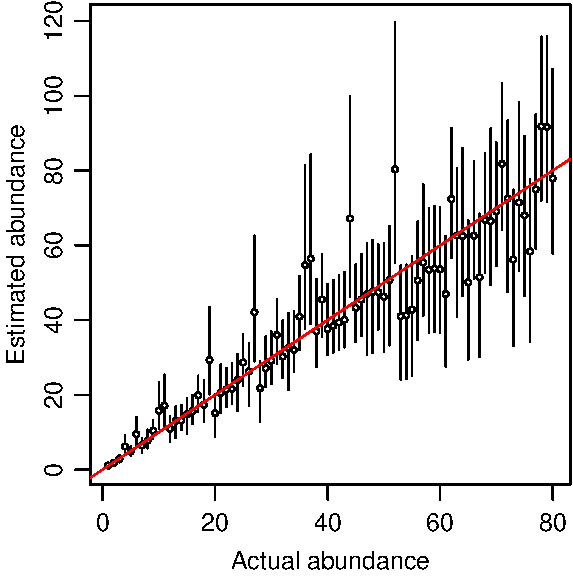
\includegraphics{modelDerivation_normPrior_files/figure-latex/fig_abundEst-1} \end{center}

Plot \(\sigma_{order}\), red line is true value:

\begin{Shaded}
\begin{Highlighting}[]
\KeywordTok{par}\NormalTok{(}\DataTypeTok{mar =} \KeywordTok{c}\NormalTok{(}\DecValTok{3}\NormalTok{, }\DecValTok{3}\NormalTok{, }\DecValTok{0}\NormalTok{, }\DecValTok{0}\NormalTok{) +}\StringTok{ }\FloatTok{0.5}\NormalTok{, }\DataTypeTok{mgp =} \KeywordTok{c}\NormalTok{(}\DecValTok{2}\NormalTok{, }\FloatTok{0.75}\NormalTok{, }\DecValTok{0}\NormalTok{))}
\KeywordTok{plot}\NormalTok{(samp[, }\StringTok{'sigCopy'}\NormalTok{], }\DataTypeTok{type =} \StringTok{'l'}\NormalTok{, }
     \DataTypeTok{xlab =} \StringTok{'Iterations'}\NormalTok{, }\DataTypeTok{ylab =} \KeywordTok{expression}\NormalTok{(sigma[orders]))}
\KeywordTok{abline}\NormalTok{(}\DataTypeTok{h =} \NormalTok{ordSD, }\DataTypeTok{col =} \StringTok{'red'}\NormalTok{)}
\end{Highlighting}
\end{Shaded}

\begin{center}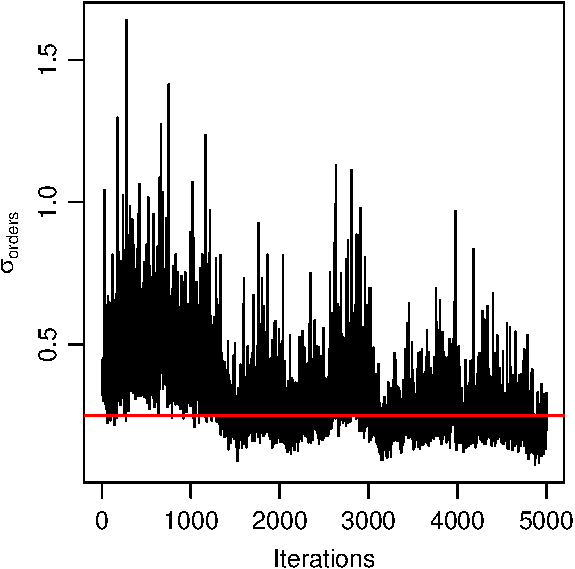
\includegraphics{modelDerivation_normPrior_files/figure-latex/fig_sigOrd-1} \end{center}


\end{document}
